\documentclass[a4paper, 12pt]{article}
\usepackage[T1]{fontenc}
\usepackage{lmodern}
\usepackage{color}
\usepackage{amsfonts}
\usepackage{epstopdf}
\usepackage{matlab}
%\documentclass{book}
\usepackage{blindtext}
\usepackage{hyperref}
\usepackage[brazil]{babel}
\usepackage{amssymb}
\usepackage[utf8]{inputenc}
\usepackage{amsmath}
\usepackage{indentfirst}
\usepackage{graphicx}
\usepackage{multicol,lipsum}
\usepackage[a4paper,
top=3cm, left=3cm, bottom=3cm, right=3cm]{geometry}
\usepackage{setspace}
\usepackage{multirow}
\usepackage{float}
\usepackage[dvipsnames]{xcolor}
\usepackage[table]{xcolor}
%\usepackage{pdflscape}
\usepackage[DIV=15]{typearea}
\usepackage[nottoc]{tocbibind}
\usepackage[sort,numbers]{natbib}
%\usepackage{cite}
\usepackage{matlab}

\usepackage[utf8]{inputenc}
\usepackage[T1]{fontenc}
\usepackage{lmodern}
\usepackage{graphicx}
\usepackage{color}
\usepackage{hyperref}
\usepackage{amsmath}
\usepackage{amsfonts}
\usepackage{epstopdf}
\usepackage[table]{xcolor}
\usepackage{matlab}


\documentclass[letterpaper]{article}
% bib pack %%%%%%%%%%%%%%%%%%%%%%%%%%%%%%%%%%%%%%%%%%%%%%%%%%%%%%%%%%%%%%%%%%%%%
\usepackage[utf8]{inputenc}
\usepackage{geometry}
    \geometry{left=3cm,right=2cm,top=2cm,bottom=2cm}
%
\usepackage[spanish]{babel}
%
\usepackage[fixlanguage]{babelbib}
    \bibliographystyle{babunsrt}
%
\usepackage{url}

\begin{document}
%\maketitle

\begin{titlepage}
	\begin{center}
		

\vspace{10pt}
%\begin{figure}[H][!ht]
%\centering
%
\includegraphics{puc-rio-logo.png}

%\end{figure}
\begin{figure}[!ht]
\centering

\includegraphics{images/puc-rio-logo.png}
\end{figure}
\huge{Dinâmica de Sistemas}
        \vspace{70pt}
        
		\textbf{ENG1730}
		\textbf{\large{\\ }}
		
		\vspace{30pt}
		\textbf{\small{\\Lista 02}}
		\vspace{75pt}
		
	\end{center}
	
	\begin{flushleft}
		\begin{tabbing}
			Aluno(a)\qquad\qquad\=\>Paloma Fernanda Loureiro Sette - 1621595\\
			
			Professor(a)\>João Carlos Virgolino Soares\\
	\end{tabbing}
		  
	\end{flushleft}
	\begin{center}
		%\vspace{\fill}
		\vspace{215pt}
		Rio de Janeiro, 13 de Setembro de 2022
	\end{center}
\end{titlepage}
%%%%%%%%%%%%%%%%%%%%%%%%%%%%%%%%%%%%%%%%%%%%%%%%%%%%%%%%%%%
\newpage
\tableofcontents
\thispagestyle{empty}

\newpage
\pagenumbering{arabic}

\newpage

%\newcommand{\listequationsname}{Lista de Equações}
%\newlistof{myequations}{equ}{\listequationsname}
%\newcommand{\myequations}[1]{%
%\addcontentsline{equ}{myequations}{\protect\numberline{\theequation}#1}\par}

%\listofmyequations
\newpage


\newpage

\listoffigures
\thispagestyle{empty}

\newpage
%%%%%%%%%%%%%%%%%%%%%%%%%%%%%%%%%%%%%%%%%%%%%%%%%%%%%%%%%
%%%%%%%%%%%%%%%%%%%%%%%%%%%%%%%%%%%%%%%%%%%%%%%%%%%

\newpage

\thispagestyle{empty}

\newpage

\section{Introdução}
Este relatório refere-se ao segundo trabalho da disciplina de Dinâmica de Sistemas, ENG1730, de 2022.2. 

Trataremos de modelagem e simulações de sistemas mecânicos massa-mola-amortecedor, utilizando Simulink e MATLAB, de acordo com a programação do curso.

\section{Questão 01}
Para a resolução dos seguintes itens que se encontram separados por subtópicos, consideremos a figura a seguir, que mostra um sistema massa-mola-amortecedor com massa \textbf{m} atrelada a duas molas e dois amortecedores.

\begin{figure}[H]
\centering

\includegraphics[scale = 0.8]{images/q01.png}
\label{filtro1}
\caption{Sistema massa-mola-amortecedor - questão 01}
\end{figure}

\subsection{Modelo matemático do sistema}

A princípio, fizemos o diagrama de corpo livre para análise das forças do sistema.

\begin{figure}[H]
\centering
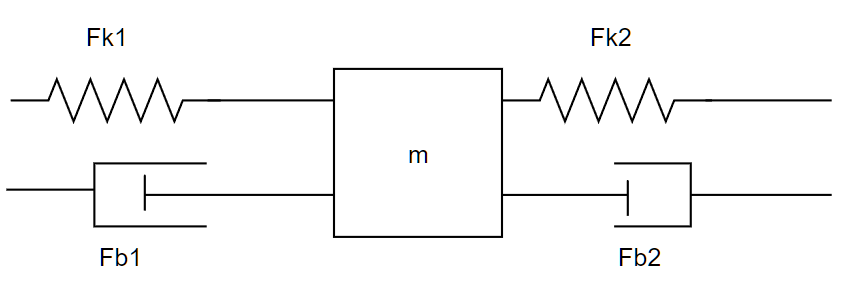
\includegraphics[scale = 0.6]{images/Q1_L2_sistema.png}
\label{filtro1}
\caption{Sistema}
\end{figure}


\begin{figure}[H]
\centering
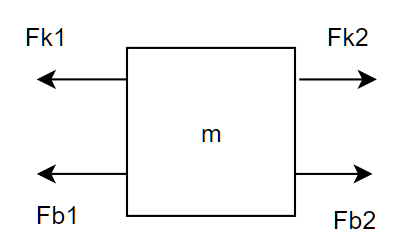
\includegraphics[scale = 0.5]{images/L2_Q1_DCL.png}
\label{filtro1}
\caption{Diagrama de Corpo Livre}
\end{figure}

Então, modelamos o sistema matematicamente:

\begin{equation}
    F_{b1} = b_1\dot x
\end{equation}

\begin{equation}
    F_{b2} = b_2\dot x
\end{equation}


\begin{equation}
    F_{k1} = k_1 x
\end{equation}


\begin{equation}
    F_{k2} = k_2 x
\end{equation}

\begin{equation}
    \sum{\vec{F}} = \vec{F_{k2}} + \vec{F_{b2}} - \vec{F_{k1}} - \vec{F_{b1}} = m\ddot x
\end{equation}

Entao,

\begin{equation}
    m\ddot x = b_2\dot x + k_2x - b_1\dot x - k_1x 
\end{equation}

\begin{equation}
    m\ddot x = \dot x(b_2 - b_1) + x(k_2 - k_1)
\end{equation}\\

Logo, o modelo matemático do sistema é representado pela equação \ref{model_mat}:

\begin{equation}\label{model_mat}
    \ddot x = \frac{1}{m} (\dot x(b_2 - b_1) + x(k_2 - k_1))
\end{equation}

\subsection{Resposta Dinâmica}
Com base no modelo matemático obtido no tópico anterior, encontramos a resposta dinâmica do sistema (posição bloco em função do tempo) utilizando o Simulink.

\begin{figure}[H]
\centering
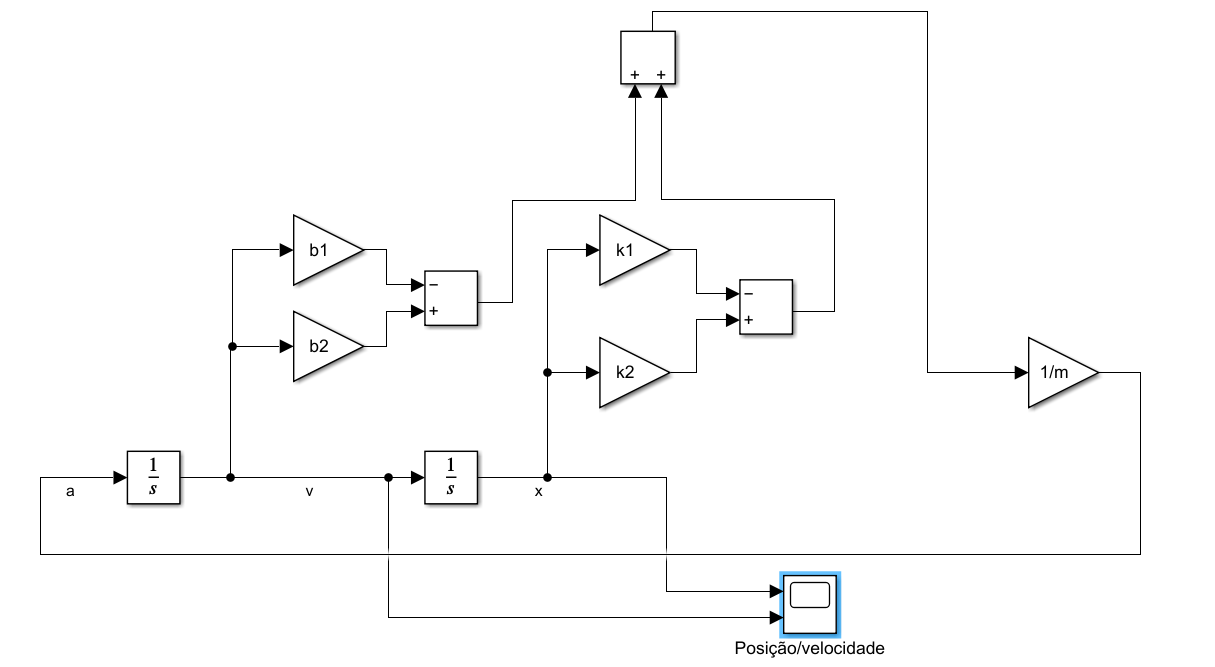
\includegraphics[scale = 0.5]{images/Q1_L2_simulink_resposta-din.png}
\label{filtro1}
\caption{Sistema modelado com o Simulink}
\end{figure}

\subsection{Definição dos Parâmetros}
% This LaTeX was auto-generated from MATLAB code.
% To make changes, update the MATLAB code and export to LaTeX again.

No MATLAB, criamos um script para a definição dos parâmetros do sistema que foi compilado no Simulink.

\sloppy
\epstopdfsetup{outdir=./}
\graphicspath{ {./L01_Latex_images/} }


\begin{matlabcode}
%% Lista 2 - questão 1
close all
clear
clc

%definição dos parâmetros

% Sistema massa-mola-amortecedor

x0 = 0.5;  % posição inicial (m)
v0 = 0;    % velocidade inicial (m/s)
k1 = 40;  % N/m
k2 = 100;  % N/m
b1 = 20; % Ns/m
b2 = 10;  % Ns/m
m = 55;     % kg

\end{matlabcode}



\subsection{Resposta Gráfica}
No script criado, devemos gerar os gráficos de posição/velocidade do bloco em função do tempo, usando os seguintes parâmetros iniciais:\\


$x_{0} = 0.5m;$\\
$v_{0} = 0m/s$\\
$k1 = 50N/m;$\\
$k2 = 100N/m;$\\
$b1 = 10Ns/m;$\\
$b2 = 5Ns/m;$\\ 
$m = 35kg$\\  



Portanto, nosso script no MATLAB apenas conteve as alterações dos valores dos parâmetros, como é visto abaixo:

% This LaTeX was auto-generated from MATLAB code.
% To make changes, update the MATLAB code and export to LaTeX again.


\sloppy
\epstopdfsetup{outdir=./}
\graphicspath{ {./L01_Latex_images/} }


\begin{matlabcode}
%% Lista 2 - questão 1
close all
clear
clc

%definição dos parâmetros

% Sistema massa-mola-amortecedor

x0 = 0.5;  % posição inicial (m)
v0 = 0;    % velocidade inicial (m/s)
k1 = 50;  % N/m
k2 = 100;  % N/m
b1 = 10; % Ns/m
b2 = 5;  % Ns/m
m = 35;     % kg

\end{matlabcode}

a resposta dinâmica do sistema (posição bloco em função do tempo) utilizando o Simulink.

\begin{figure}[H]
\centering
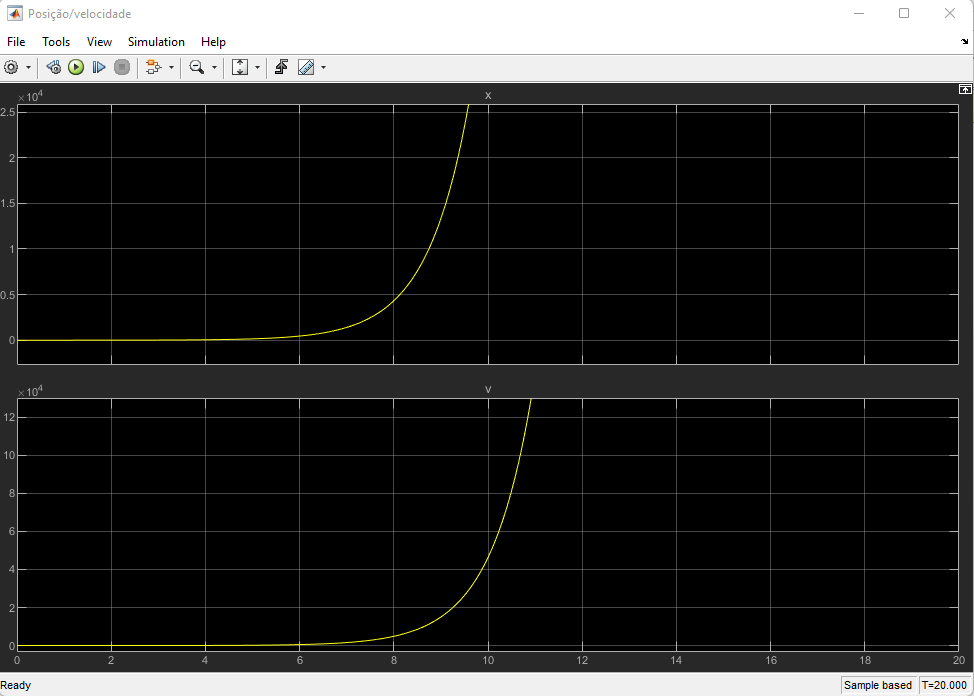
\includegraphics[scale = 0.55]{images/Q1_L2_4.png}
\label{filtro1}
\caption{Resposta gráfica com o Simulink}
\end{figure}



\subsection{Resposta Dinâmica com o Simscape}
Encontramos a resposta dinâmica do sistema utilizando, agora, o Simscape. \\

Comparando o resultado obtido no Simulink com o resultado obtido no Simscape, foi notada uma diferença com relação à resposta gráfica. Pode-se dizer que a resposta obtida com o Simscape faz mais sentido, uma vez que nosso sistema possui elemento amortecedor e o gráfico expressa uma oscilação que entende-se por um movimento harmônico amortecido.

\begin{figure}[H]
\centering
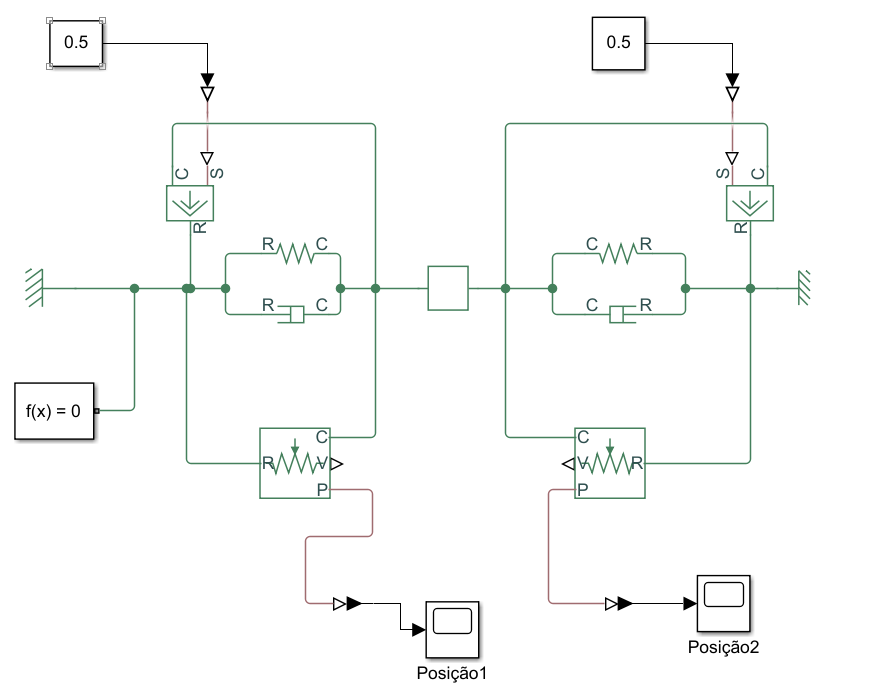
\includegraphics[scale = 0.5]{images/Q1_L2_simscape.png}
\label{filtro1}
\caption{Sistema modelado utilizando o Simscape}
\end{figure}

\begin{figure}[H]
\centering
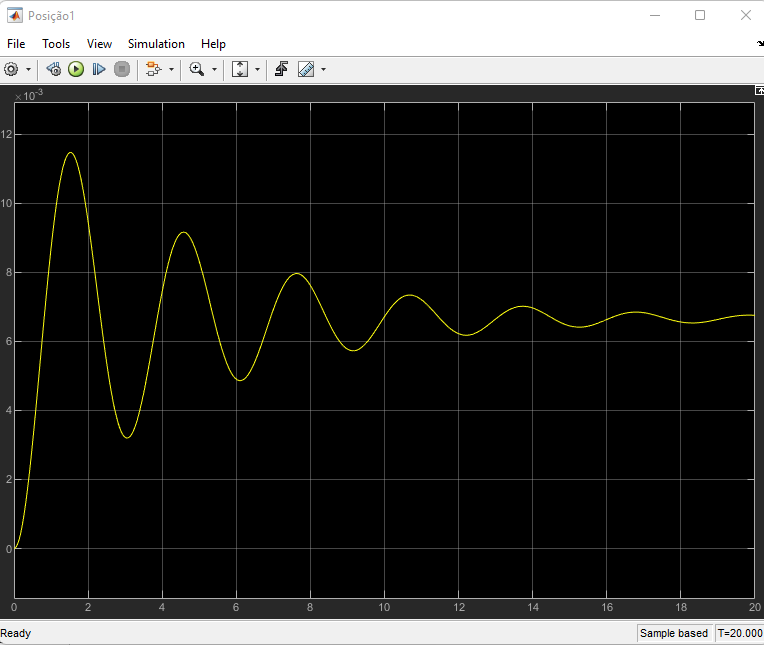
\includegraphics[scale = 0.55]{images/Q1_L2_5.png}
\label{filtro1}
\caption{Resposta gráfica do sistema com o Simscape}
\end{figure}

\subsection{Inércia do Sistema (v=0) em t < 10s}
Ao tornar o sistema inerte em menos de 10 segundos, foi reduzido o valor do parâmetro $m$, que corresponde à massa. 


\begin{figure}[H]
\centering
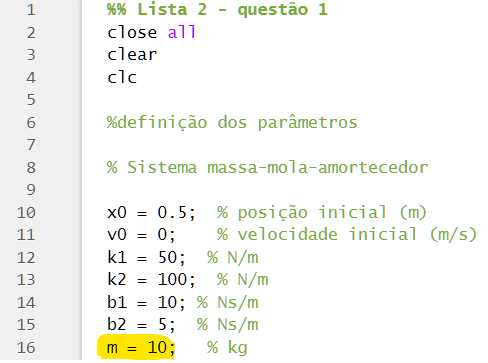
\includegraphics[scale = 0.6]{images/Q1_L2_6.2.png}
\label{filtro1}
\caption{Alteração da massa para t < 10s}
\end{figure}

\begin{figure}[H]
\centering
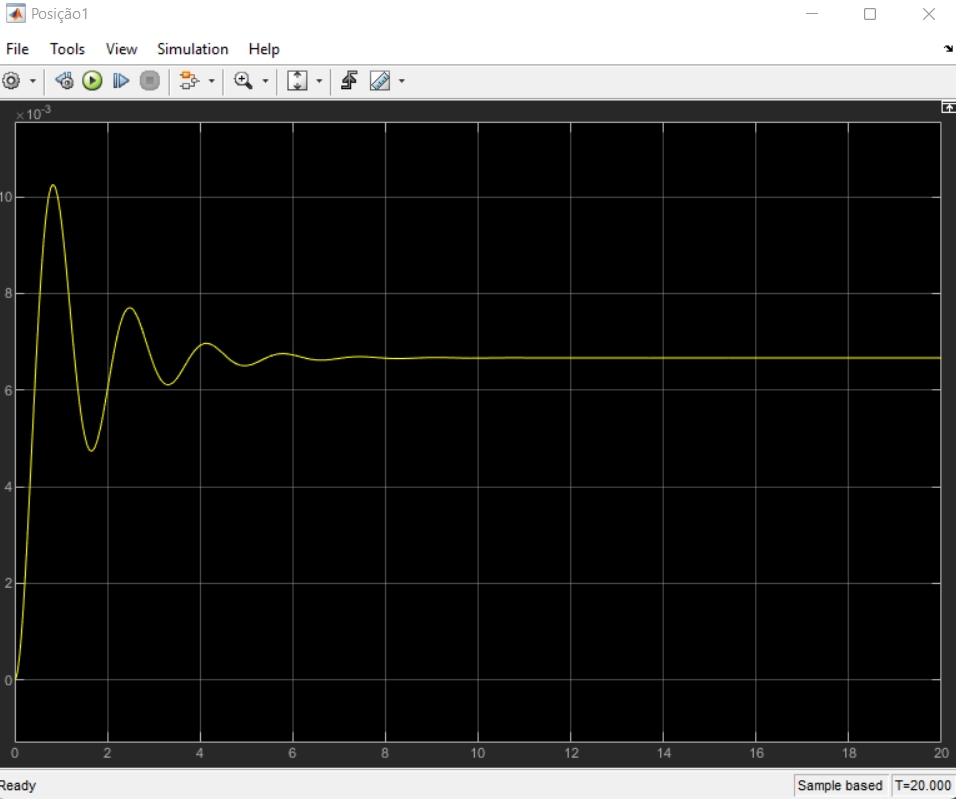
\includegraphics[scale = 0.55]{images/Q1_L2_6.png}
\label{filtro1}
\caption{Resposta gráfica após a redução para massa para v=0 em t<10s}
\end{figure}

\newpage
\section{Questão 02}

A figura a seguir mostra um sistema massa-mola-amortecedor com uma massa, uma mola e um amortecedor.

\begin{figure}[H]
\centering

\includegraphics[scale = 0.8]{images/q02.png}
\label{filtro1}
\caption{Sistema massa-mola-amortecedor - questão 02}
\end{figure}

\subsection{Modelo matemático do sistema}
Novamente, começamos pelo Diagrama de Corpo Livre:

\begin{figure}[H]
\centering
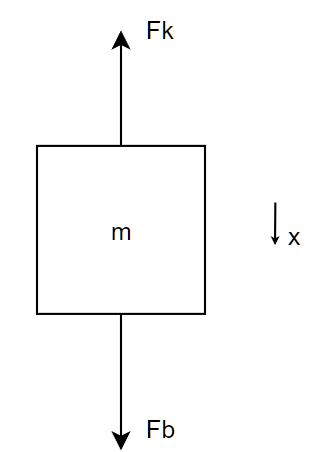
\includegraphics[scale = 0.55]{images/Q2_DCL.png}
\label{filtro1}
\caption{Diagrama de Corpo Livre - Questão 2}
\end{figure}

Teremos que,

\begin{equation}
    \sum{F} = m\ddot x = 0
\end{equation}


\begin{equation}
     m \ddot x + b\dot x  = - kx 
\end{equation}

Logo, o modelo matemático do sistema pode ser representado por

\begin{equation}
     \ddot x  = \frac{1}{m}(- kx - b\dot x) 
\end{equation}


\subsection{Resposta Dinâmica com Simulink}
A partir do modelo matematico, podemos simular a resposta dinâmica do sistema com o auxílio do Simulink.

\begin{figure}[H]
\centering
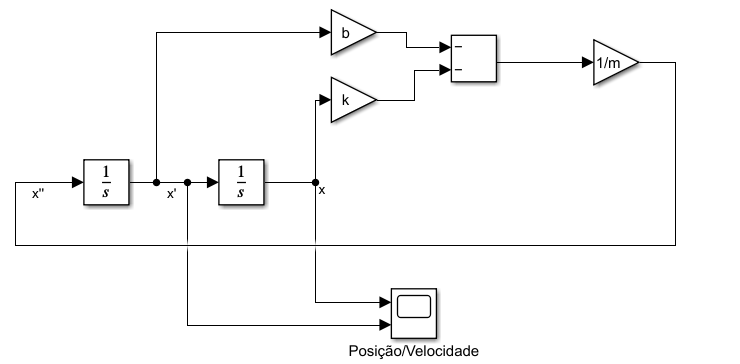
\includegraphics[scale = 0.8]{images/Q2_L2_simulink.png}
\label{filtro1}
\caption{Modelagem do sistema através do Simulink}
\end{figure}

\subsection{Definição dos Parâmetros}

Criamos, consequentemente, um script no MATLAB para utilização dos parâmetros nos elementos do sistema no Simulink.

\begin{matlabcode}
%% Lista 2 - questão 2
close all
clear
clc

%definição dos parâmetros

% Sistema massa-mola-amortecedor

x0 = 0.5;  % posição inicial (m)
v0 = 0;    % velocidade inicial (m/s)
k = 20;  % N/m
b = 4;  % Ns/m
m = 2;   % kg

\end{matlabcode}

\subsection{Resposta Gráfica}

É pedido que geremos os gráficos da posição e da velocidade em funçao do tempo utilizando os seguintes parâmetros:\\

$x_0 = 0.5 m$\\
$v_0 = 0 m/s$\\
$k = 20 N/m$\\
$b = 4 Ns/m$\\
$m = 2 kg$\\

Estes mesmos parâmetros foram utilizados durante a criação do script, como é visto no código MATLAB anexado no tópico anterior. Portanto, teremos como resposta gráfica o seguinte:


\begin{figure}[H]
\centering
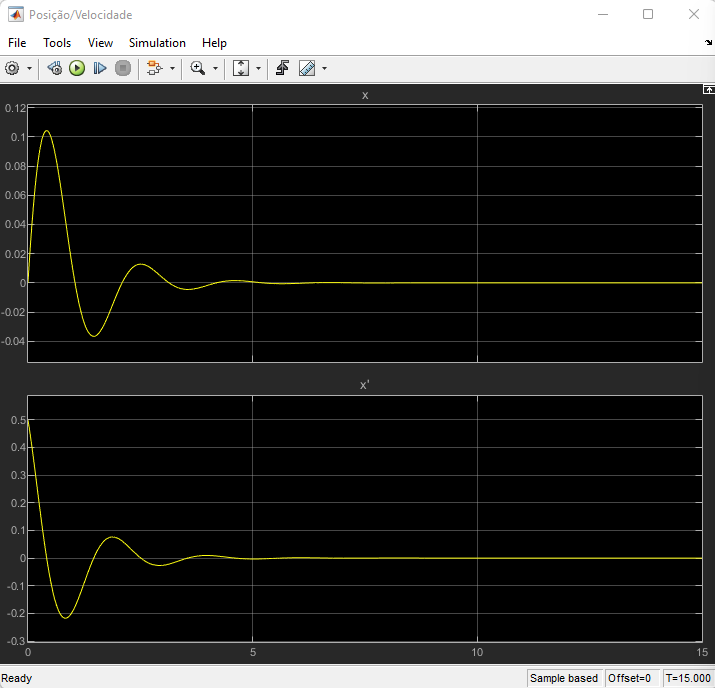
\includegraphics[scale = 0.7]{images/Q2_L2_simu_graph_4.png}
\label{filtro1}
\caption{Gráfico do posição/velocidade do sistema - Simulink}
\end{figure}

\newpage
\subsection{Resposta Dinâmica com o Simscape}

Da mesma forma, simulamos o sistema com o auxílio do Simscape, gerando posteriormente sua resposta gráfica e realizando a comparação necessária da resposta obtida com o Simulink.\\

\begin{figure}[H]
\centering
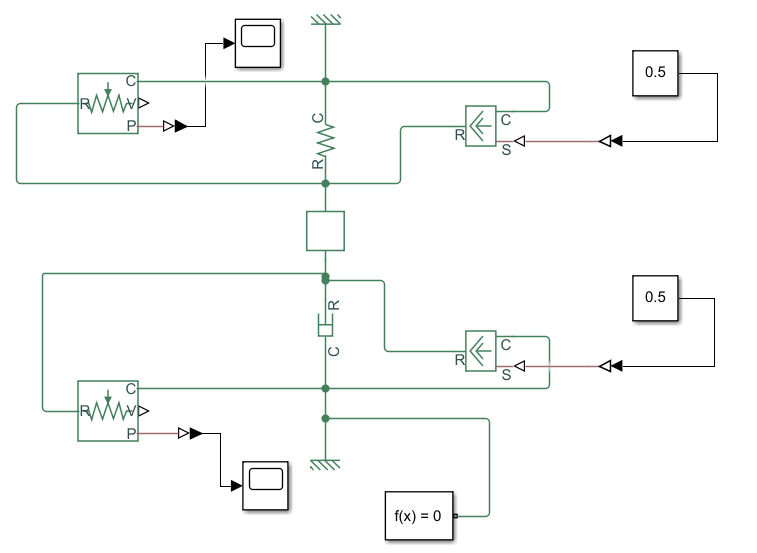
\includegraphics[scale = 0.8]{images/Q2_L2_simscape.png}
\label{filtro1}
\caption{Resposta dinâmica do sistema com o Simscape}
\end{figure}

Como era esperado, obtivemos a resposta gráfica semelhante ao que foi gerado através do Simulink, uma vez que estamos tratando do mesmo sistema em modelagens diferentes.

\begin{figure}[H]
\centering
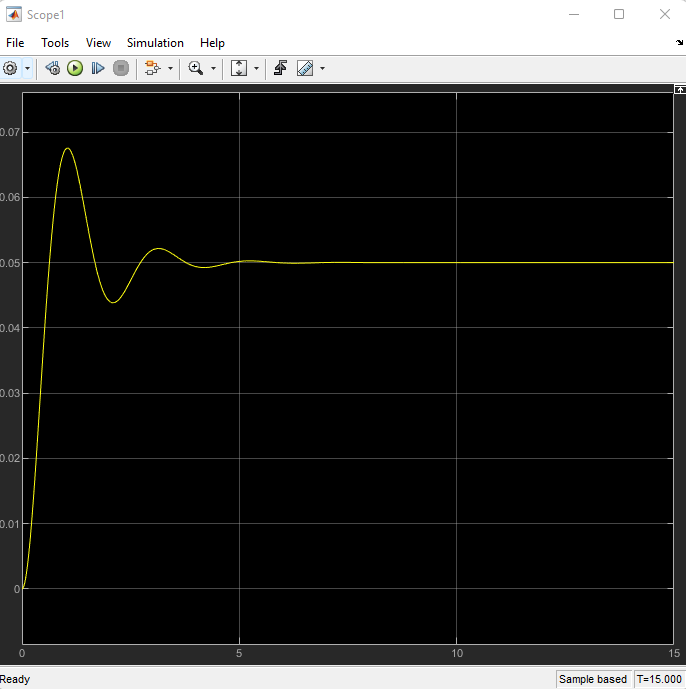
\includegraphics[scale = 0.7]{images/Q2_L2_sims_graph_.png}
\label{filtro1}
\caption{Gráfico do posição/velocidade do sistema - Simscape}
\end{figure}


\newpage
% REFERENCIAS %%%%%%%%%%%%%%%%%%%%%%%%%%%%%%%%%%%%%%%%%%%%%%%%%%%%%%%%%%%%%%
    \nocite{*}
    \bibliography{src/bibliography}
    
\end{document}
\section{Referências Bibliográficas}



\end{document}